\documentclass[tikz,border=4pt]{standalone}
\usepackage[utf8]{inputenc}
\usepackage[T1]{fontenc}
\usetikzlibrary{arrows.meta,positioning}
\definecolor{ataque}{HTML}{2a78d6}
\definecolor{defesa}{HTML}{eb6834}
\definecolor{tinta}{HTML}{52514e}
\definecolor{campo}{HTML}{eef5ec}
\begin{document}
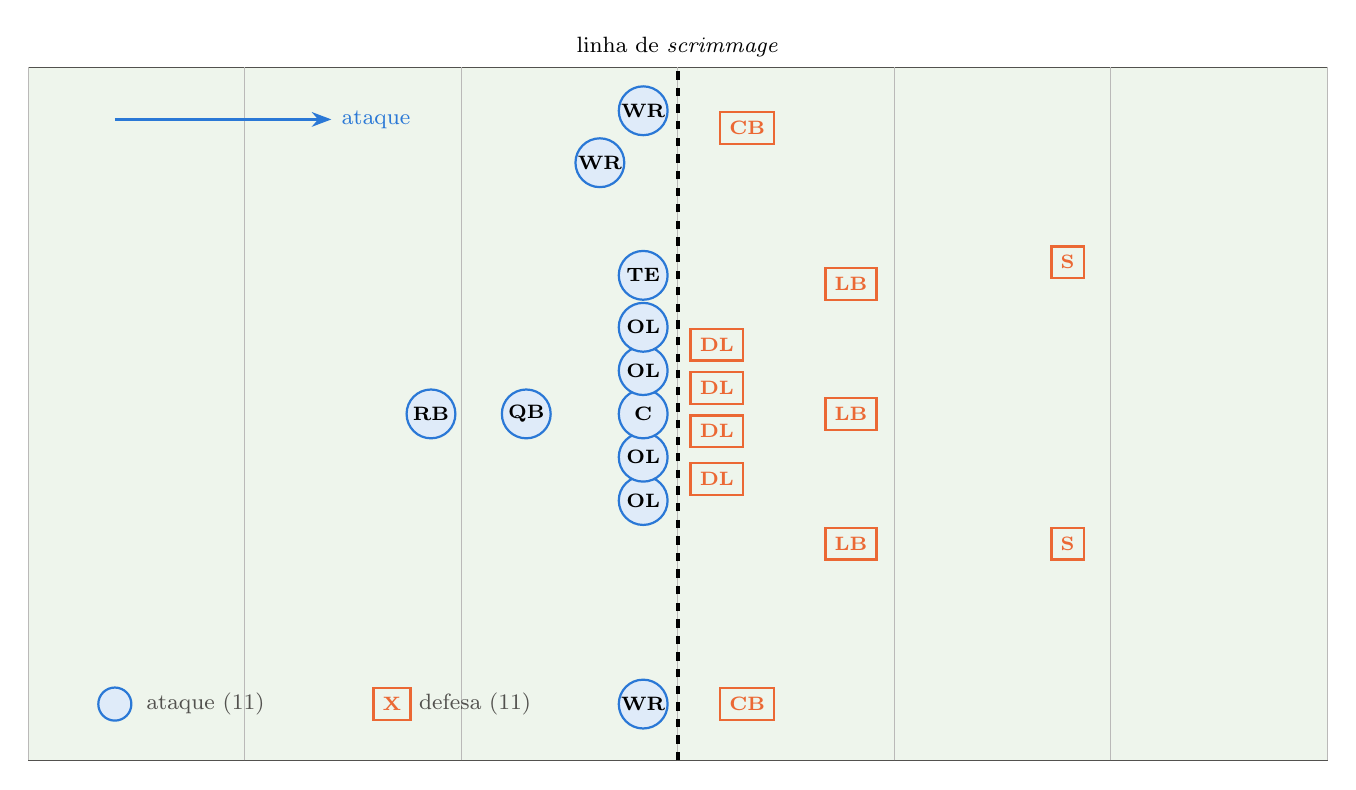
\begin{tikzpicture}[x=0.55cm,y=0.55cm,font=\footnotesize,
  atq/.style={circle, draw=ataque, fill=ataque!15, line width=0.8pt, minimum size=0.62cm, inner sep=0pt, font=\scriptsize\bfseries},
  def/.style={draw=defesa, line width=0.9pt, font=\scriptsize\bfseries, text=defesa}]
% campo (recorte de 30 jardas x largura total)
\fill[campo] (0,0) rectangle (30,16);
\draw[tinta] (0,0) rectangle (30,16);
\foreach \x in {0,5,...,30} \draw[tinta!40] (\x,0) -- (\x,16);
% linha de scrimmage
\draw[very thick, dashed, black] (15,0) -- (15,16) node[above, font=\footnotesize] {linha de \textit{scrimmage}};
% ataque (move para a direita)
\foreach \y/\l in {6/OL,7/OL,8/C,9/OL,10/OL} \node[atq] at (14.2,\y) {\l};
\node[atq] at (11.5,8) {QB};
\node[atq] at (9.3,8) {RB};
\node[atq] at (14.2,11.2) {TE};
\node[atq] at (14.2,1.3) {WR};
\node[atq] at (13.2,13.8) {WR};
\node[atq] at (14.2,15) {WR};
% defesa
\foreach \y in {6.5,7.6,8.6,9.6} \node[def] at (15.9,\y) {DL};
\foreach \y in {5,8,11} \node[def] at (19,\y) {LB};
\node[def] at (16.6,1.3) {CB};
\node[def] at (16.6,14.6) {CB};
\node[def] at (24,5) {S};
\node[def] at (24,11.5) {S};
% direcao do ataque
\draw[-{Stealth[length=2.5mm]}, thick, ataque] (2,14.8) -- (7,14.8) node[right, text=ataque] {ataque};
% legenda
\node[atq, minimum size=0.42cm] at (2.0,1.3) {}; \node[right, text=tinta] at (2.5,1.3) {ataque (11)};
\node[def] at (8.4,1.3) {X}; \node[right, text=tinta] at (8.8,1.3) {defesa (11)};
\end{tikzpicture}
\end{document}
